\chapter{Implementação}\label{chap:chap4}

% \section*{}
% Este capítulo pode ser dedicado à apresentação de detalhes de nível
% mais baixo relacionados com o enquadramento e implementação das
% soluções preconizadas no capítulo anterior.
% Note-se no entanto que detalhes desnecessários à compreensão do
% trabalho devem ser remetidos para anexos.

% Dependendo do volume, a avaliação do trabalho pode ser incluída neste
% capítulo ou pode constituir um capítulo separado.

A ideia principal do projeto seria fazer a deteção de objetos simples e depois capitalizar nessa capacidade desenvolvida para fazer a deteção de objetos mais complexos. Esta deteção de objetos, que culminou na escolha da mesa como caso de estudo, pelas considerações que já foram explanadas da sua morfologia, tem como objetivo último a sua utilização num demonstrador de robótica autónoma, fazendo recurso a um dicionário pré-existente em que as mesas conhecidas são listadas num ficheiro \emph{XML}.

O programa desenvolvido foi escrito em \emph{C++} recorrendo a algumas bibliotecas informáticas, nomeadamente a \emph{Point Cloud Library} (PCL) para a captura e manipulação de nuvens de pontos e a \emph{Boost} porque além de ser um requisito da PCL tem uma miríade de bibliotecas auxiliares implementadas que potenciam o desenvolvimento e trazem uma garantia de terem a melhor performance possível. De seguida são analisados com mais detalhe os pormenores de implementação.

\section{Captura de Imagens 3D para análise }

A captura de imagens em 3D foi desenvolvida utilizando a biblioteca \emph{Point Cloud Library}, e é uma das opções do projeto associado a esta dissertação. As nuvens de pontos são guardadas em ficheiros PCD e guardam o que é capturado pelo \emph{Kinect}, sendo que contém toda a informação RGBD e pode ser visualizada com a mesma aplicação que as gerou.

\begin{center}
	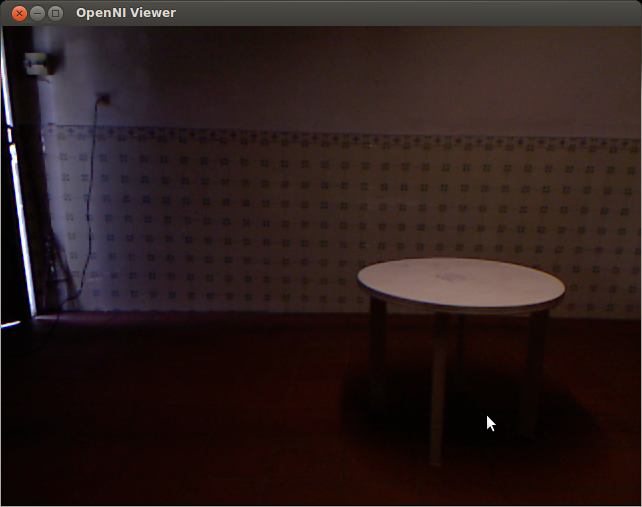
\includegraphics[width=0.8\textwidth]{figures/experiencia/exp4.png}\\
	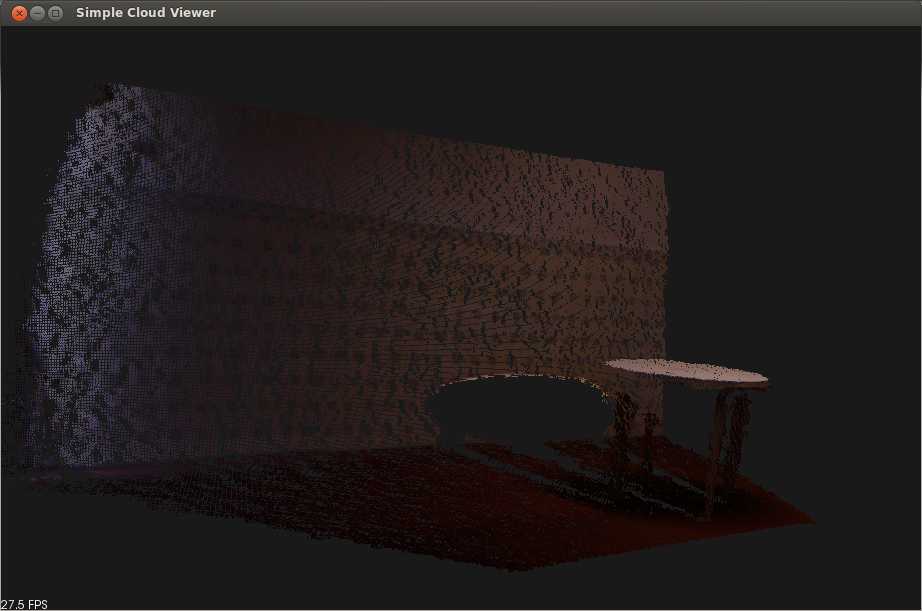
\includegraphics[width=0.4\textwidth]{figures/exemplo_captura_perspectiva1.png}
	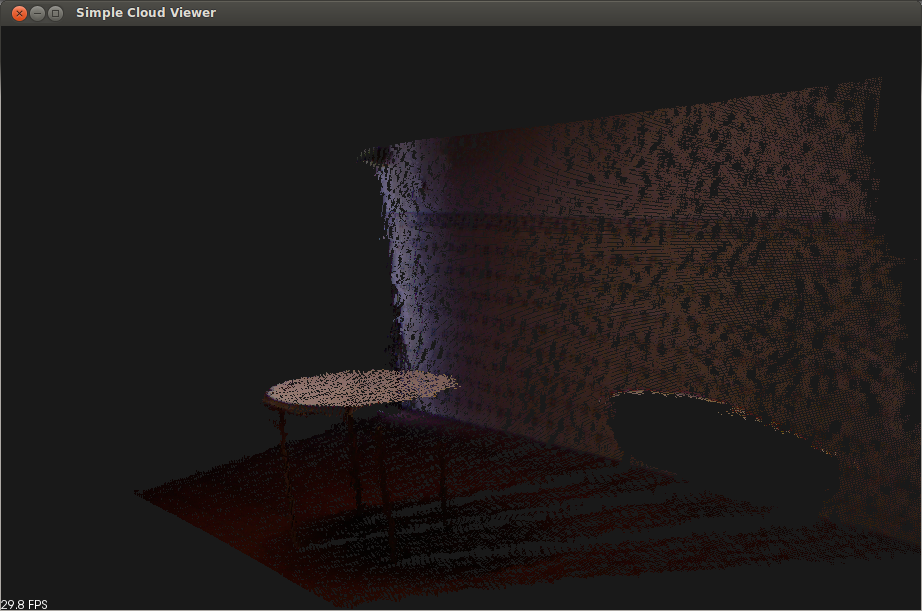
\includegraphics[width=0.4\textwidth]{figures/exemplo_captura_perspectiva2.png}

	\captionof{figure}{Exemplo de imagem capturada com informação RGBD (duas perspetivas) e a imagem RGB correspondente.}
	\label{fig:exemplo_captura}
\end{center}

\subsection{Análise seleção e Separação de amostra de controlo}

Selecionou-se imagens com mesas para testar a qualidade de deteção após o desenvolvimento da tese, para avaliar a adequação da solução ao problema.


\section{Estudo de Precisão do Kinect}

Antes de se passar à implementação da deteção, considerou-se necessário fazer um estudo da precisão das medições do Kinect de modo a garantir que as análises a imagens e qualquer consideração prévia estariam corretas e não se baseavam em suposições.

Sendo assim escolheu-se um objeto e mudou-se a sua posição relativa ao \emph{Kinect}. Em cada uma das posições registadas, foram medidas e guardadas as distâncias e os ângulos, sendo que de seguida foram registadas doze imagens RGBD por posição e submeteu-se cada uma a uma análise automatizada para medir a distância e o ângulo ao objeto.

A sequencia dos registos encontra-se na tabela~\ref{res:dist_analise} que se encontra abaixo.

\begin{table}[htb]
	\begin{center}
		\begin{tabular} { l c c c}
			Nº da Posição & Distância & Ângulo \\
			\hline
			1 & 1.35 & 0 \\
			2 &  1.34 & 21\\
			3 & 2.00 & 0 \\
			4 & 1.93 & 14 \\
			5 & 2.30 & -27\\
			6 & 2.75 & 0 \\
			7 & 2.75 & 18 \\
			8 & 3.00 & -18 \\
			\hline
		\end{tabular}
		\caption{Experiências à precisão do Kinect}
		\label{res:dist_analise}
	\end{center}
\end{table}

A posição da mesa relativamente ao \emph{Kinect} para cada posição pode ser verificado na figura~\ref{fig:exp_posicoesmesa}.

\begin{center}
	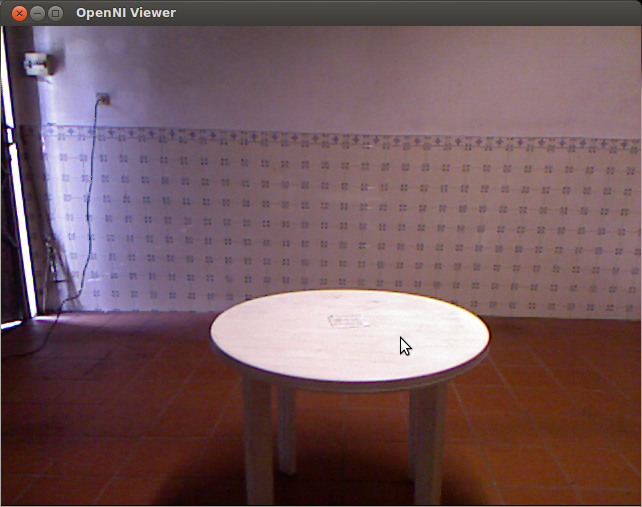
\includegraphics[width=0.240\textwidth]{figures/experiencia/exp1.png}
	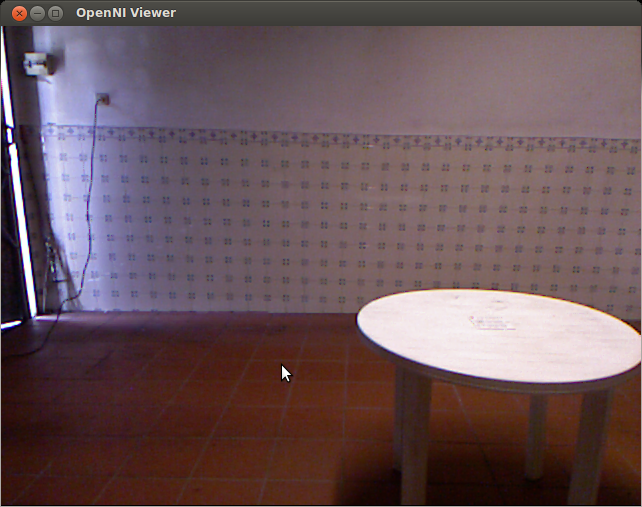
\includegraphics[width=0.240\textwidth]{figures/experiencia/exp2.png}
	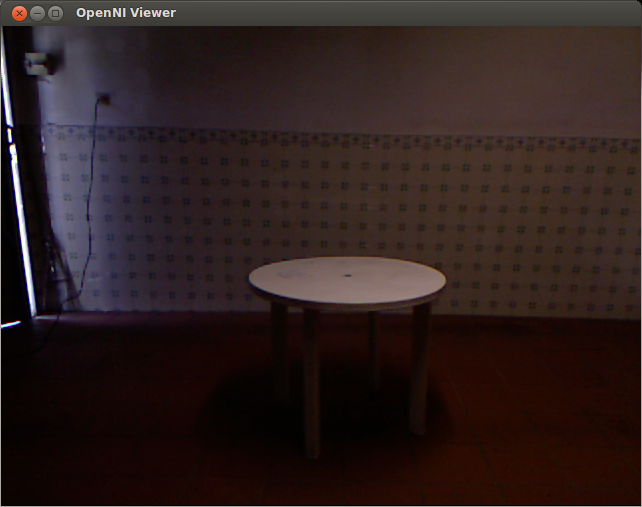
\includegraphics[width=0.240\textwidth]{figures/experiencia/exp3.png}
	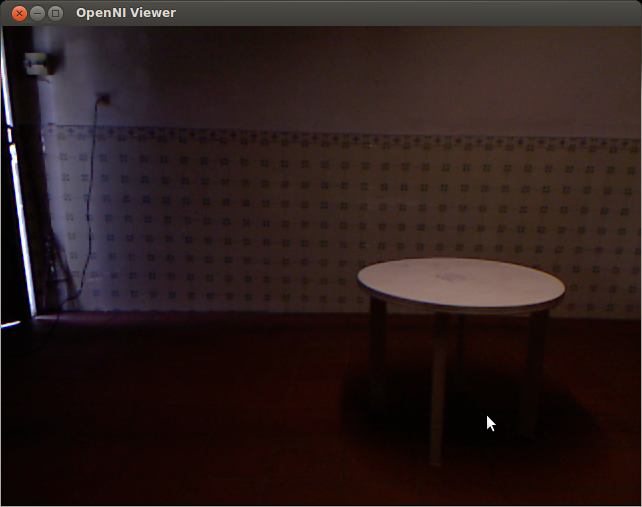
\includegraphics[width=0.240\textwidth]{figures/experiencia/exp4.png} \\
	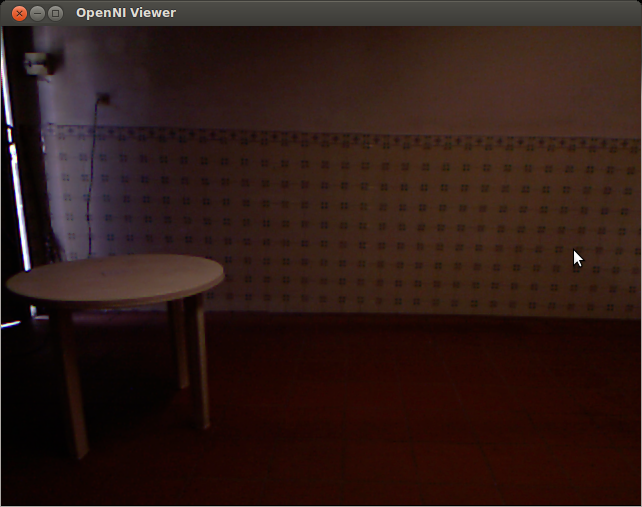
\includegraphics[width=0.240\textwidth]{figures/experiencia/exp5.png}
	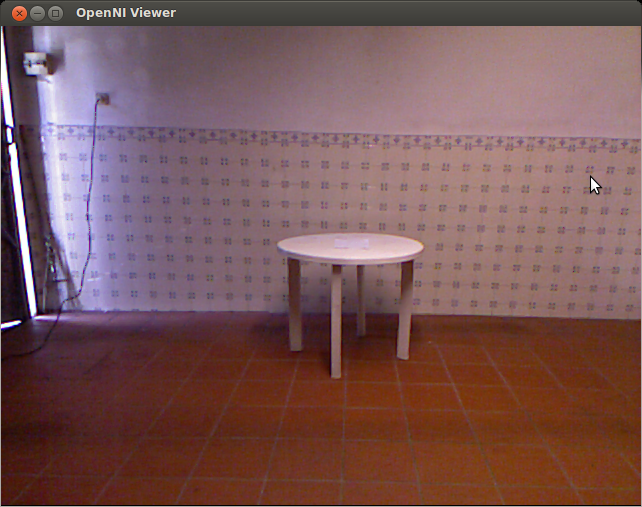
\includegraphics[width=0.240\textwidth]{figures/experiencia/exp6.png}
	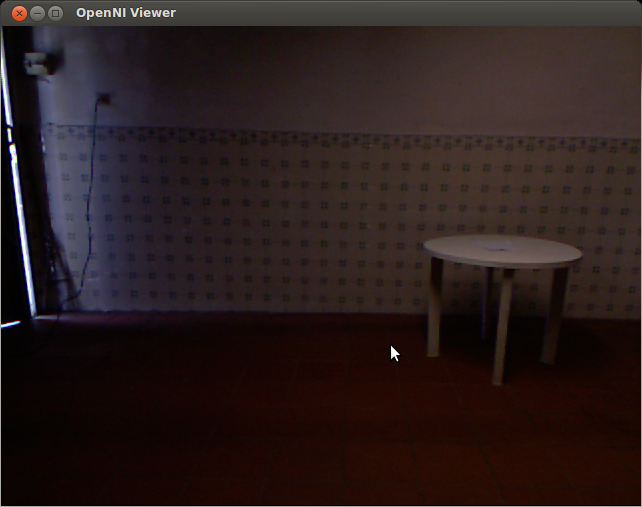
\includegraphics[width=0.240\textwidth]{figures/experiencia/exp7.png}
	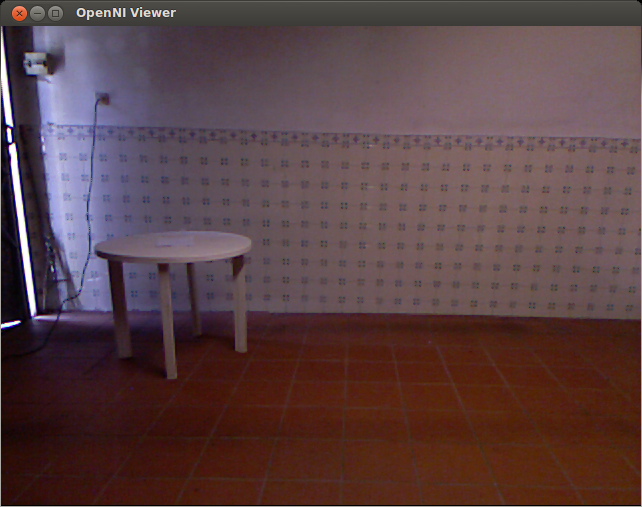
\includegraphics[width=0.240\textwidth]{figures/experiencia/exp8.png}
	\captionof{figure}{Foto das posições da mesa relativas ao Kinect.}
	\label{fig:exp_posicoesmesa}
\end{center}


De seguida para cada imagem de cada posição avaliou-se qual a distância do \emph{Kinect} à mesa que a imagem RGBD regista. Os resultados encontram-se registados na tabela~\ref{res:exp_res_obtidos} sendo que para cada uma das posições criou-se um diagrama temporal para avaliar quanto as posições registada pelo \emph{Kinect} se desviam da posição medida fisicamente, que se encontram apresentados abaixo.


\begin{table}[!h]
\begin{center}
\begin{tabular} { c c c c c c c c }

\hline
\multicolumn{8}{c}{ Posições }\\
\hline
 1 & 2 & 3 & 4 & 5 & 6 & 7 & 8 \\
\hline
1.35 & 1.339247 & 1.975414 & 1.910938 & 2.413945 & 2.762543 & 2.753629 & 3.023028 \\
1.35754 & 1.334866 & 1.952989 & 1.931228 & 2.377091 & 2.76339 & 2.750247 & 3.060131 \\
1.362351 & 1.334632 & 1.985518 & 1.931326 & 2.38616 & 2.786931 & 2.771791 & 3.059977 \\
1.35799 & 1.339735 & 1.985523 & 1.931682 & 2.36845 & 2.786493 & 2.791635 & 3.062525 \\
1.358089 & 1.339071 & 1.975026 & 1.931579 & 2.380317 & 2.791077 & 2.771245 & 3.059977 \\
1.35759 & 1.339247 & 1.974677 & 1.930731 & 2.380086 & 2.78675 & 2.770061 & 3.042213 \\
1.357634 & 1.334736 & 1.985874 & 1.942546 & 2.380075 & 2.786312 & 2.791803 & 3.044104 \\
1.358572 & 1.338895 & 1.987369 & 1.931143 & 2.344773 & 2.812669 & 2.813004 & 3.04185 \\
1.358485 & 1.334144 & 1.987345 & 1.931502 & 2.351119 & 2.786493 & 2.791803 & 3.04185 \\
1.355191 & 1.339556 & 1.974662 & 1.931858 & 2.376915 & 2.700064 & 2.771245 & 3.02285 \\
1.358148 & 1.339383 & 1.98587 & 1.942116 & 2.353092 & 2.790619 & 2.817074 & 3.02285 \\
1.357711 & 1.339069 & 1.98587 & 1.942461 & 2.348412 & 2.720287 & 2.794201 & 3.022684 \\
\hline
\end{tabular}
	\caption{Resultados obtidos das distâncias para cada posição}
	\label{res:exp_res_obtidos}
\end{center}
\end{table}


\begin{figure}
\begin{center}
	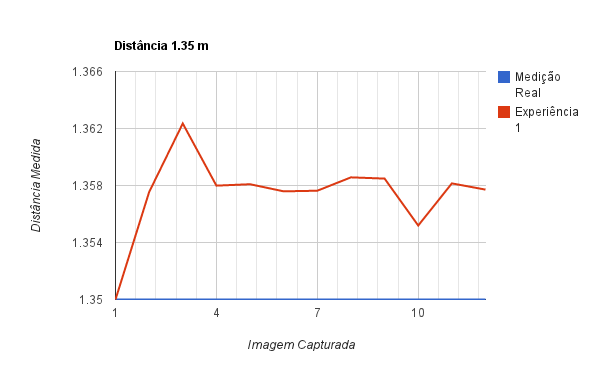
\includegraphics[width=0.80\textwidth]{figures/experiencia/chart_1.png}
	\captionof{figure}{Diagrama temporal para a primeira posição (1.35 m)}
	\label{fig:chart_1}
\end{center}
\end{figure}

\begin{figure}
\begin{center}
	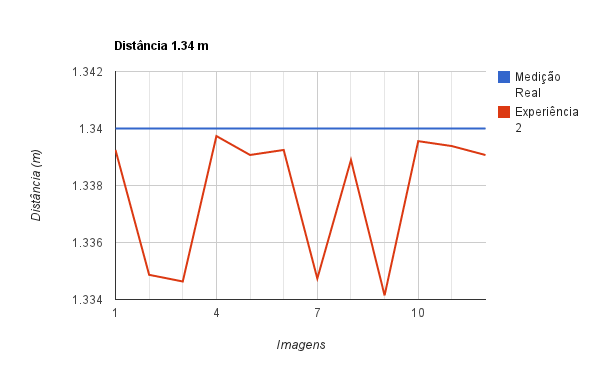
\includegraphics[width=0.80\textwidth]{figures/experiencia/chart_2.png}
	\captionof{figure}{Diagrama temporal para a primeira posição (1.34 m)}
	\label{fig:chart_2}
\end{center}
\end{figure}

\begin{figure}
\begin{center}
	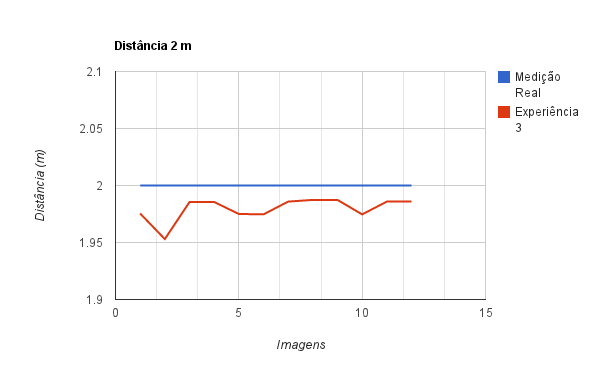
\includegraphics[width=0.80\textwidth]{figures/experiencia/chart_3.png}
	\captionof{figure}{Diagrama temporal para a primeira posição (2.00 m)}
	\label{fig:chart_3}
\end{center}
\end{figure}

\begin{figure}
\begin{center}
	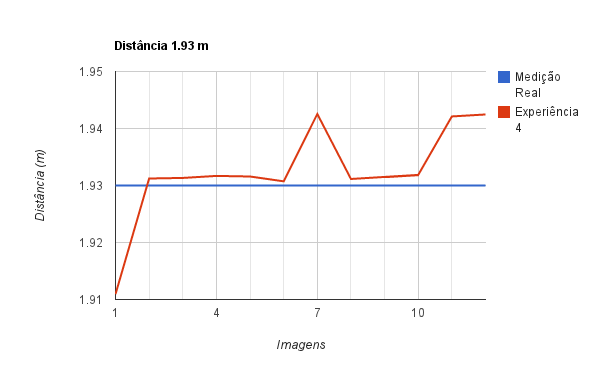
\includegraphics[width=0.80\textwidth]{figures/experiencia/chart_4.png}
	\captionof{figure}{Diagrama temporal para a primeira posição (1.93 m)}
	\label{fig:chart_4}
\end{center}
\end{figure}

\begin{figure}
\begin{center}
	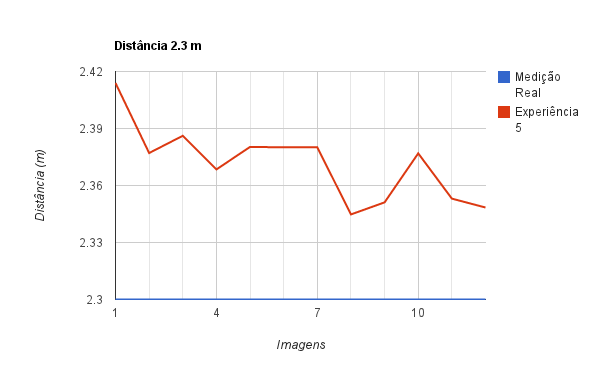
\includegraphics[width=0.80\textwidth]{figures/experiencia/chart_5.png}
	\captionof{figure}{Diagrama temporal para a primeira posição (2.30 m)}
	\label{fig:chart_5}
\end{center}
\end{figure}

\begin{figure}
\begin{center}
	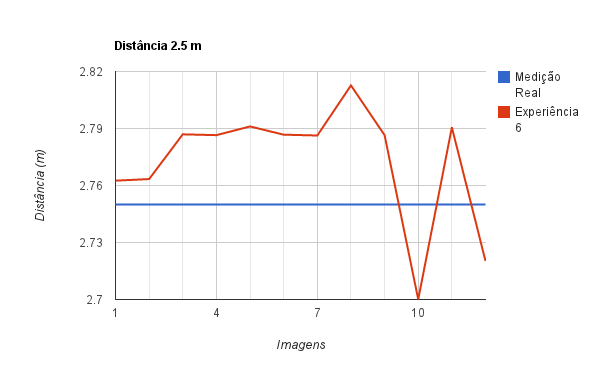
\includegraphics[width=0.80\textwidth]{figures/experiencia/chart_6.png}
	\captionof{figure}{Diagrama temporal para a primeira posição (2.75 m)}
	\label{fig:chart_6}
\end{center}
\end{figure}

\begin{figure}
\begin{center}
	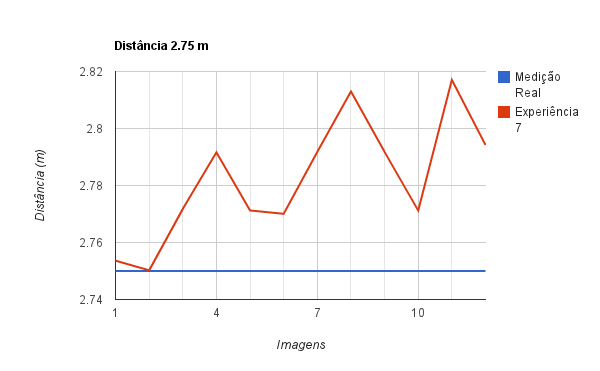
\includegraphics[width=0.80\textwidth]{figures/experiencia/chart_7.png}
	\captionof{figure}{Diagrama temporal para a primeira posição (2.75 m)}
	\label{fig:chart_7}
\end{center}
\end{figure}

\begin{figure}
\begin{center}
	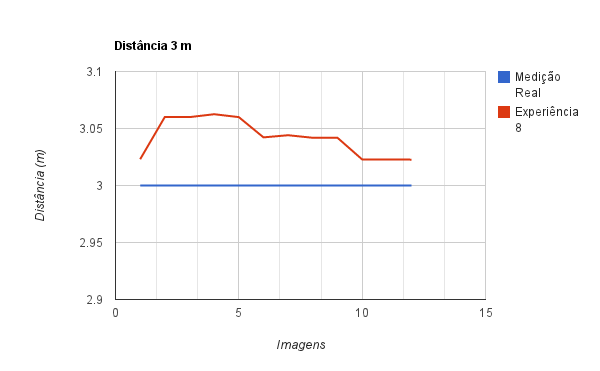
\includegraphics[width=0.80\textwidth]{figures/experiencia/chart_8.png}
	\captionof{figure}{Diagrama temporal para a primeira posição (3.00 m)}
	\label{fig:chart_8}
\end{center}
\end{figure}

Para aprofundar a análise, extraiu-se alguns dados estatísticos das medições que se encontram na tabela~\ref{res:exp_res_obtidos_est} 


\begin{table}[h!]
\begin{center}
\begin{tabular} { c c c c }
Posição & Média & Desvio Padrão & Mediana \\
\hline
1 & 1.3574 & 0.0017 & 1.3579 \\
2 & 1.3377 & 0.0024 & 1.3391\\
3 & 1.9797 & 0.0104 & 1.9855 \\
4 & 1.9324 & 0.0051 & 1.9315 \\
5 & 2.3717 & 0.0154 & 2.3770 \\
6 & 2.7728 & 0.0336 & 2.7865 \\
7 & 2.7823 & 0.0200 & 2.7817 \\
8 & 3.0420 & 0.0157 & 3.0420 \\
\hline
\end{tabular}
	\caption{Dados estatísticos da recolha de distâncias.}
	\label{res:exp_res_obtidos_est}
\end{center}
\end{table}

Olhando para o desvio padrão, percebe-se que a variação dos dados do \emph{Kinect} para a posição do objeto não é muito grande, sendo no máximo de 2 centímetros, contudo houve uma variação algo significativa para o valor medido mas não era demasiado grande, sendo que se considerou bastante aceitável.


Quanto aos ângulos, fez-se uma análise semelhante à das distâncias, cujos resultados são os apresentados nas tabelas \ref{res:exp_res_obtidos_ang} e \ref{res:exp_res_obtidos_est_ang}.

\begin{table}[!htb]
\begin{center}
\begin{tabular} { c c c c c c c c }

\hline
 \multicolumn{8}{c}{ Posições }\\
\hline
1 & 2 & 3 & 4 & 5 & 6 & 7 & 8 \\
\hline
 -15.357386 & 4.792201 &-9.630516 & 4.790509 & -34.3685 & -4.143964 & 14.146553 & -25.240545 \\
 -15.223657 & 4.976701 & -9.608464 & 4.506991 & -34.520763 & -4.379865 & 13.799928 & -24.792519 \\
 -15.168276 & 4.835194 & -9.448602 & 4.506991 & -34.371037 & -4.460659 & 13.811712 & -24.792519 \\
 -15.301353 & 4.932463 & -9.449469 & 4.63898 & -34.216621 & -4.343729 & 13.708774 & -24.889385\\
 -15.301353 & 4.700834 & -9.563814 & 4.63898 & -34.165874 & -5.161427 & 13.811712 & -24.792519\\
 -15.223657 & 4.792201 & -9.501884 & 4.317291 & -34.626232 & -4.460659 & 13.69715 & -25.071798\\
 -15.238359 & 4.994671 & -9.510148 & 4.612736 & -34.626232 & -4.343729 & 13.708774 & -25.169027\\
 -15.383727 & 4.584675 & -9.765748 & 4.476339 & -37.209705 & -5.005285 & 13.602537 & -25.071798\\
 -15.370365 & 4.740714 & -9.761795 & 4.607438 & -34.071758 & -4.343729 & 13.708774 & -25.071798\\
 -15.642712 & 4.926197 & -9.501012 & 4.738488 & -34.981014 & -4.604316 & 13.811712 & -25.240545\\
15.318219 & 4.861241 & -9.511069 & 4.451008 & -34.617245 & -5.044734 & 13.94077 & -25.240545\\
-15.250415 & 4.563166 & -9.511069 & 4.581371 & -33.973186 & -4.329277 & 13.935993 & -25.240545\\

\hline
\end{tabular}
	\caption{Resultados obtidos das distâncias para cada posição}
	\label{res:exp_res_obtidos_ang}
\end{center}
\end{table}



\begin{table}[h!]
\begin{center}
\begin{tabular} { c c c c }
 Posição & Média & Desvio Padrão & Mediana \\
\hline
	1 & -15.3150 &0.1279 & -15.3014 \\
	2 & 4.8084 &0.1491 & 4.8137 \\
	3 &  -9.5636 &0.1114 &-9.5111\\
	4 &  4.5723 &0.1152 & 4.5944 \\
	5 & -34.6457 &0.8926 &-34.4459 \\
	6 & -4.5518 & 0.3215 &-4.4203 \\
	7 & 13.8070 & 0.1034 &  13.8058 \\
	8 & -25.0511 & 0.1861 &  -25.0718 \\
\hline
\end{tabular}
	\caption{Dados estatísticos da recolha de ângulos.}
	\label{res:exp_res_obtidos_est_ang}
\end{center}
\end{table}


\begin{table}[h!]
\begin{center}
\begin{tabular} { c c c c }
 Posição & Valor Real & Mediana & |Valor Real - Mediana| \\
\hline
	1 & 0 & -15.3014 & 15.3014 \\
	2 & 21 & 4.8137 & 16.1863 \\
	3 & 0 & -9.5111& 9.5111\\
	4 & 14 & 4.5944 & 9.4056\\
	5 & -27 & -34.4459 & 7.4459 \\
	6 & 0 & -4.4203 & 4.4203 \\
	7 & 18 & 13.8058 & 4.1942 \\
	8 & -18 & -25.0718 & 7.0718 \\
\hline
\end{tabular}
	\caption{Comparação do valor da mediana com o valor real.}
	\label{res:exp_res_obtidos_est_ang_comp}
\end{center}
\end{table}



Comparando o valor da mediana dos valores obtidos pelo \emph{Kinect} aos que foram fisicamente medidos (ver tabela~\ref{res:exp_res_obtidos_est_ang_comp}), consegue-se concluir que a diferença absoluta entre ambos é no máximo 15 graus, o que aliado aos baixo valores do desvio padrão (< 1 grau) é um indicador que o dispositivo é bastante preciso. 

Olhando para os resultados, é possível também afirmar que a medição física dos ângulos provavelmente não estaria completamente alinhada com o foco do \emph{Kinect}.

\vspace*{12mm}


\section {Implementação da Deteção}

Agora serão listados todos os passos por que passa uma imagem RGBD para se poder detetar a existência de mesas na nuvem de pontos.

Antes de tudo a informação RGB é descartada pois não tem uma grande influência sobre deteção, isto porque após considerações cuidadosas chegou-se à conclusão que a cor não é um aspeto que tenha grande peso na caracterização da mesa.

Adicionalmente o dicionário de mesas conhecidas é lido a partir do ficheiro \emph{dictionary.xml} e guardado em memória para se poder fazer a comparação com o que é encontrado na imagem e dar um valor que avalia a confiança com que pode garantir que é a mesa indicada.


\begin{figure}[h!]
	\begin{center}
	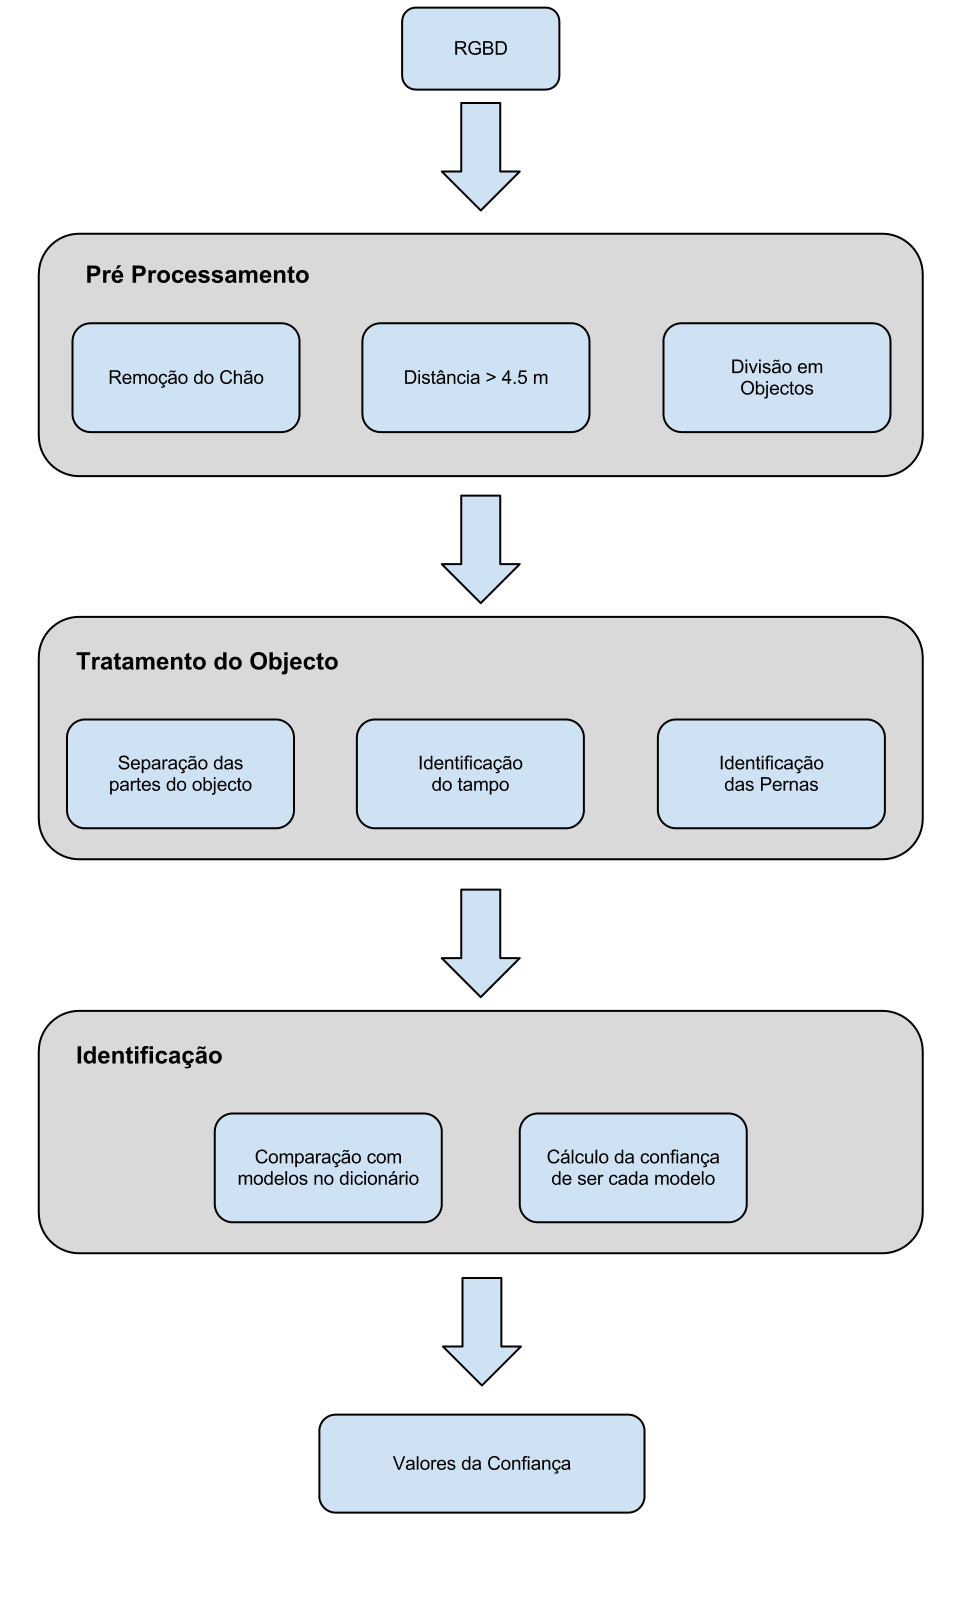
\includegraphics[width=0.80\textwidth]{figures/processo_identificacao.png}
		\captionof{figure}{Funcionamento do processo global.}
		\label{fig:processamento}
	\end{center}
\end{figure}

\vspace*{12mm}



O ficheiro de dicionário, onde se podem descrever as mesas do dicionário, tem a seguinte gramática:

\begin{description}
	\item [table] - Este é o nó principal que contém os nós com as descrições da mesa;
	\item [name] - Onde é guardado o nome representativo da mesa;
	\item [top] - Onde estão contidos os atributos do tampo que tem a seguinte estrutura:
	\begin{description} 
		\item [shape] - Palavra descritiva da forma do tampo da mesa;
		\item [large\_dimension] - A maior distância medida no tampo em metros; 
		\item [small\_dimension] - A menor distância medida no tampo em metros;
	\end{description} 
	\item [legs] - Onde estão contidos os atributos das pernas da mesa que tem os seguintes parâmetros:
	\begin{description} 
		\item [number] - O número de pernas que a mesa tem;
		\item [height] -  A altura das pernas em metros;
		\item [parallel] - Se as pernas são paralelas ou não;
		\item [center\_distance] - distância das pernas ao centro da mesa.
	\end{description} 
\end{description}

Em suma, as características das mesas são distribuídas entre o tampo da mesa e as pernas, descrevendo a sua morfologia em tanto parâmetros quantitativos como a altura e dimensões dos tampos como em parâmetros qualitativos como a geometria do tampo e se as pernas são paralelas.


\subsection{Pré Processamento}

Agora que se trabalha sobre a informação de profundidade, que se encontra em SI (metros), é feito um pré processamento onde se descarta tudo que aparece na imagem que dista a mais de 4,5 metros do sensor. Isto é no sentido de eliminar erros persistentes na imagem, pois o \emph{Kinect} vai perdendo precisão com a distância \cite{s120201437}. No passo seguinte vai-se remover o maior plano que corresponde ao chão, de modo a isolar os objetos que se encontrem na imagem.


Depois é feita uma clusterização usando o algoritmo de vizinhança Euclidiana para separar o que resta da imagem em objetos coerentes e separáveis. Isto, dando um exemplo prático, é para não acontecer o caso de estarmos a reconhecer o que parece uma perna de uma mesa a dois metros de distância do que é reconhecido como um tampo.

No final deste pré processamento o resultado será um conjunto de nuvens de pontos, em que cada uma representa um objeto que se encontra na imagem capturada inicial.

\begin{figure}[htb]
\begin{center}
	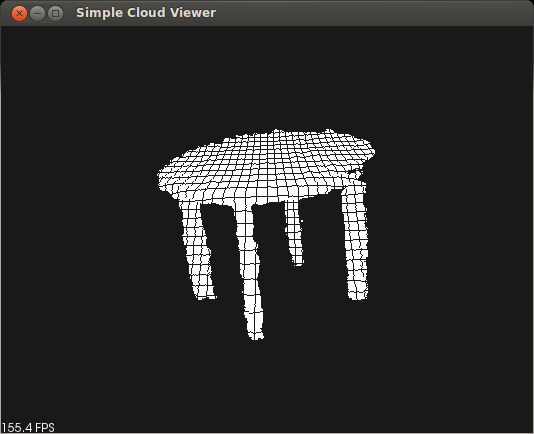
\includegraphics[width=0.80\textwidth]{figures/mesa1_1.png}
	\captionof{figure}{Exemplo de imagem após pré processamento.}
	\label{fig:exemplo_processado}
\end{center}
\end{figure}

\subsection{Deteção de Mesas}

De seguida cada um dos objetos separados passa por um processo onde se tenta 
detetar constituintes das mesas, como pernas e tampos. Caso sejam encontrados 
verifica-se se correspondem a alguma das mesas conhecidas que estão guardadas
no dicionário das mesas conhecidas, retornando um valor de de confiança \(C\) que se encontra sempre entre 0 e 1.

Esta deteção é feita nos seguintes passos: primeiro faz-se a deteção do tampo, que é obrigatoriamente uma superfície planar, e caso não tenha um plano é logo atribuída uma confiança de 0, considerando-se que não é uma mesa.

Caso exista um plano, então existe um tampo e as suas dimensões são avaliadas e comparadas com cada um dos modelos. Para avaliar a confiança (\(C_t\)) de o tampo da mesa ser o do modelo que está no dicionário, é seguida a seguinte formulação para cada uma das características (\(C_i\)):

\begin{equation}\label{eq:ci}
C_i = 1 - \frac{|valor\_modelo - valor\_observado|}{valor\_modelo}
\end{equation}

Sendo que se avalia tanto a dimensão maior \(C_1\) como a mais pequena  \(C_2\) e são ambas igualmente relevantes para a avaliação do ajuste da mesa observada vão ter ambas um peso de 0.5 na avaliação do tampo, portanto o valor da confiança \(C_t\) é calculado através da seguinte fórmula:

\begin{equation}\label{eq:ct}
C_t = 0.5C_1 + 0.5C_2
\end{equation}

De seguida é feita uma análise aos apoios, cuja confiança é representada por \(C_a\) sendo que tem em consideração o número de apoios observados, e a altura dos mesmos. Cada um destes fatores, respetivamente \(C_n\) e \(C_h\), são computados seguindo a formulação~\ref{eq:ci}. Os valores obtidos são pesados onde a \(C_n\) é aplicado um fator de 0.4 pois facilmente um dos apoios é oculto nas imagens em 3D portanto tem de ter um peso menor, enquanto que a altura \(C_h\) dos apoios tem um peso de 0.6 na avaliação de os apoios corresponderem aos do modelo no dicionário. Em termos de fórmula:

\begin{equation}\label{eq:ca}
C_a = 0.4C_n + 0.6C_h
\end{equation}


Com base no que foi detetado o valor de confiança global é calculado, distribuindo a confiança igualmente pelo que foi calculado quanto ao tampo \(C_t\) e e quanto aos apoios \(C_a\) sendo que a formulação final fica:

\begin{equation}\label{eq:cfinal}
C = 0.5C_t + 0.5C_a
\end{equation}

De seguida analisa-se os resultados que são produzidos pela metodologia descrita.

\section {Resultados Obtidos}

Para se obter resultados foram analisadas três mesas diferentes que são descritas no seguinte ficheiro de dicionário em XML. 

\begin{verbatim}
dictionary.xml

<?xml version="1.0" ?>
<table>
	<name>Mesa 1</name>
	<top shape="round" large_dimension="0.89" small_dimension="0.89"/>
	<legs  number="4" height="0.68" parallel="true"/>
</table>
<table>
	<name>Mesa 2</name>
	<top shape="squared" large_dimension="1.0" small_dimension="1.0"/>
	<legs  number="4" height="0.7" parallel="true"/>
</table>
<table>
	<name>Mesa 3</name>
	<top shape="squared" large_dimension="1.0" small_dimension="1.0"/>
	<legs  number="4" height="0.59" parallel="true"/>
</table>
<table>
	<name>Mesa 4</name>
	<top shape="squared" large_dimension="2.0" small_dimension="1.5"/>
	<legs  number="3" height="0.9" parallel="true"/>
</table>
<table>
	<name>Mesa 5</name>
	<top shape="round" large_dimension="1.5" small_dimension="1.5"/>
	<legs  number="1" height="0.8" parallel="true" />
</table>
\end{verbatim}

E captou-se uma série de imagens RGBD em várias perspetivas dessas mesas para tentar fazer o reconhecimento.

A primeira mesa, apresentada na figura~\ref{fig:mesa1}, como aparece representado no dicionário, é uma mesa redonda, com aproximadamente 90 centímetros de diâmetro e tem quatro apoios com cerca de 70 centímetros de altura.

\begin{figure}[htb]
\begin{center}
	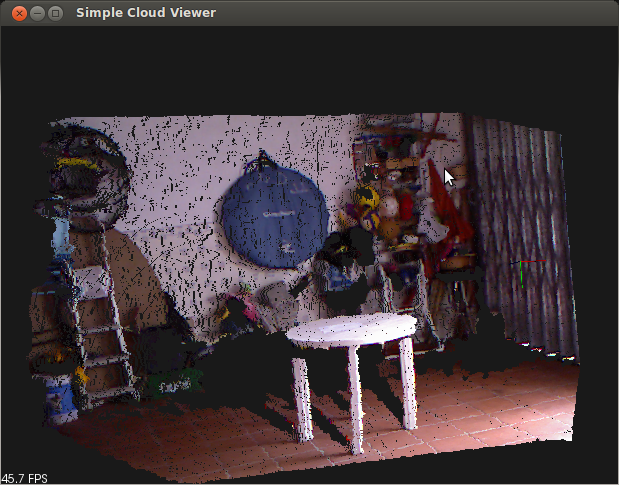
\includegraphics[width=0.80\textwidth]{figures/exemplo_captura.png}
	\captionof{figure}{Primeira mesa a ser identificada.}
	\label{fig:mesa1}
\end{center}
\end{figure}

A segunda mesa a ser identificada é idêntica à primeira mas tem um tampo quadrado de 1 metro de lado, como pode ser observado na figura.

\begin{figure}[htb]
\begin{center}
	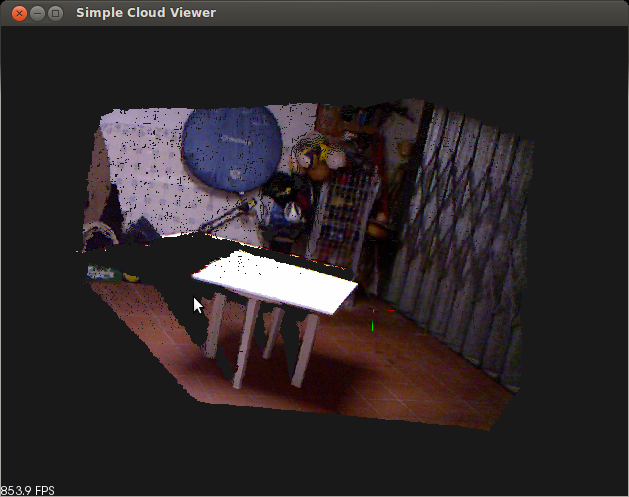
\includegraphics[width=0.80\textwidth]{figures/mesa2.png}
	\captionof{figure}{Segunda mesa a ser identificada.}
	\label{fig:mesa2}
\end{center}
\end{figure}

A terceira mesa é mais baixa com cerca de 60 centímetros de altura e tem quatro apoios. O tampo é quadrado e tem 1 metro de lado.
\begin{figure}[htb]
\begin{center}
	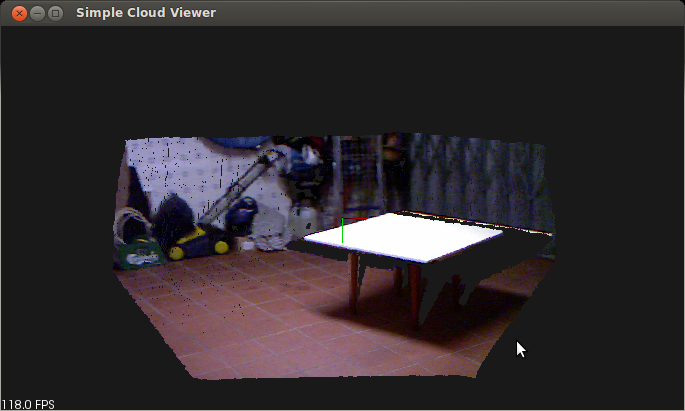
\includegraphics[width=0.80\textwidth]{figures/mesa3.png}
	\captionof{figure}{Terceira mesa a ser identificada.}
	\label{fig:mesa3}
\end{center}
\end{figure}

As mesas 3 e 4 não correspondem a mesas testadas, contudo servem para analisar como é que esta metodologia de reconhecimentos avalia morfologias diferentes.

\begin{table}[htb]
\begin{center}
\begin{tabular} { l | c c c }
	\multicolumn{4}{ c }{ Comparação das mesas}\\
	\hline
	Característica & Mesa 1 & Mesa 2 & Mesa 3 \\
	\hline
	Forma & Circular & Quadrada & Quadrada \\
	Dimensão Maior do Tampo  & 0.89 & 1.0 & 1.0 \\
	Dimensão Menor do Tampo & 0.89 & 1.0 & 1.0 \\
	Numero de Pernas & 4 & 4 & 4 \\
	Altura & 0.68 & 0.7 & 0.59 \\
	Pernas Paralelas & sim & sim & sim \\
	\hline
\end{tabular}
	\caption{Comparação das dimensões das mesas analisadas.}
	\label{res:mesas_comp}
\end{center}
\end{table}


Os resultados da identificação para cada uma das mesas descritas são apresentados abaixo, sendo que antes se apresenta a significância de cada uma das variáveis:

\begin{itemize}
	\item \(C_1\) - Confiança da dimensão maior;
	\item \(C_2\) - Confiança da dimensão menor;
	\item \(C_n\) - Confiança do número de pernas;
	\item \(C_h\) - Confiança da altura das pernas;
	\item \(C\) - Confiança de ter identificado a mesa analisada;
\end{itemize}


De seguida seguem-se os resultados das experiências feitas, sendo que de uma série de imagens RGBD das três mesas diferentes foram escolhidas três e verificou-se se era possível identificar a mesa correta através da metodologia proposta. É também de notar que as experiências foram realizadas num computador com um processador \emph{Core i7-2630QM} e 4GB  de memória.

\subsection{Identificação}

\begin{table}[htb]
%\caption{Mesa 1}
\begin{center}
\begin{tabular} { c c c c c | c }
	\hline
	Modelo do dicionário & \(C_1\) & \(C_2\) & \(C_n\) & \(C_h\) & \(C\) \\
	\hline
	\multicolumn{6}{ c }{Primeiro Ensaio}\\
	\hline
	Mesa 1 &	 0.997753 &	0.987125 & 1.000000 & 0.702837 & 0.907070 \\
	Mesa 2 &	 0.892000 &	0.878541 & 1.000000 & 0.682756 & 0.847462 \\
	Mesa 3 &	 0.892000 &	0.878541 & 1.000000 & 0.810049 & 0.885650 \\
	Mesa 4 &	 0.446000 &	0.585694 & 0.666667 & 0.531032 & 0.550567 \\
	Mesa 5 &	 0.594667 &	0.585694 & -2.000000 & 0.597411 & 0.074314 \\
	\hline
	\multicolumn{6}{ c }{Segundo Ensaio}\\
	\hline
	Mesa 1 &	 0.938588 &	0.816854 & 0.750000 & 0.785464 & 0.824500 \\
	Mesa 2 &	 0.835343 &	0.727000 & 0.750000 & 0.763022 & 0.769492 \\
	Mesa 3 &	 0.835343 &	0.727000 & 0.750000 & 0.905281 & 0.812170 \\
	Mesa 4 &	 0.417671 &	0.484667 & 1.000000 & 0.593462 & 0.603623 \\
	Mesa 5 &	 0.556895 &	0.484667 & -1.000000 & 0.667645 & 0.260684 \\
	\hline
	\multicolumn{6}{ c }{Terceiro Ensaio}\\
	\hline
	Mesa 1 &	 0.986337 &	0.946067 & 1.000000 & 0.607531 & 0.865360 \\
	Mesa 2 &	 0.902160 &	0.842000 & 1.000000 & 0.590173 & 0.813092 \\
	Mesa 3 &	 0.902160 &	0.842000 & 1.000000 & 0.700205 & 0.846102 \\
	Mesa 4 &	 0.451080 &	0.561333 & 0.666667 & 0.459023 & 0.524144 \\
	Mesa 5 &	 0.601440 &	0.561333 & -2.000000 & 0.516401 & 0.045614 \\
	\hline
\end{tabular}
	\caption{Resultados das análises da Mesa 1}
	\label{res:mesa1}
\end{center}
\end{table}

A análise de uma imagem RGBD da Mesa 1 apresenta resultados bastante satisfatórios, onde o modelo do dicionário com um valor de confiança mais alto é o que na realidade a representa nas três experiências. Verificou-se também que existe pouca diferença entre o valor de confiança do modelo da Mesa 1 e o da Mesa 2, contudo poderá ser explicável pelo facto de as duas mesas com morfologias muito aproximadas.



Adicionalmente os \emph{clusters} representativas das mesas encontram-se na figura~\ref{fig:mesa1_ensaios}.

\begin{figure}[htb]
\begin{center}
	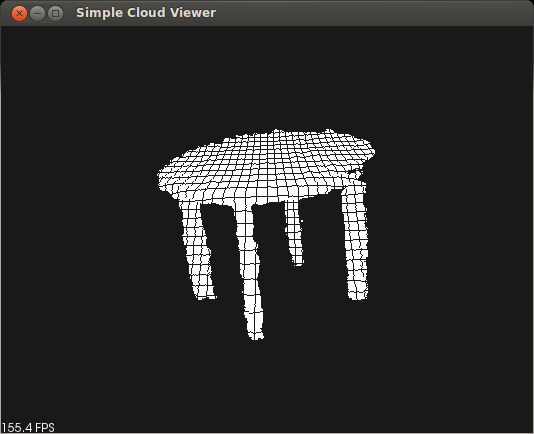
\includegraphics[width=0.30\textwidth]{figures/mesa1_1.png}
	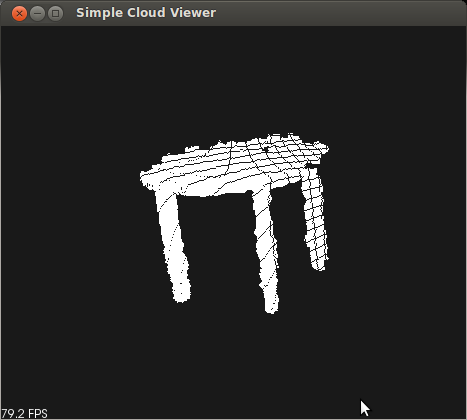
\includegraphics[width=0.30\textwidth]{figures/mesa1_2.png}
	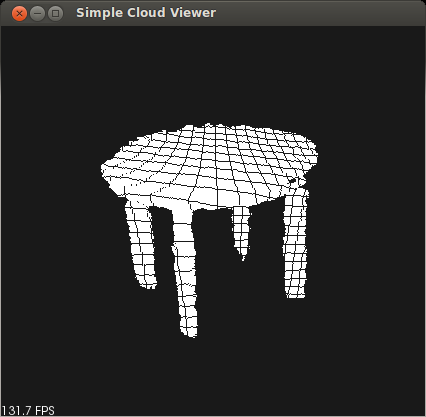
\includegraphics[width=0.30\textwidth]{figures/mesa1_3.png}
	\captionof{figure}{Clusters representativos da mesa 1.}
	\label{fig:mesa1_ensaios}
\end{center}
\end{figure}

\begin{table}[htb]
\begin{center}
\begin{tabular} { c c c c c | c }
	Modelo do dicionário & \(C_1\) & \(C_2\) & \(C_n\) & \(C_h\) & \(C\) \\
		\hline
	\multicolumn{6}{ c }{Primeiro Ensaio}\\
	\hline
	Mesa 1 &	 0.622630 &	0.789887 & 1.000000 & 0.647027 & 0.747238 \\
	Mesa 2 &	 0.774141 &	0.923000 & 1.000000 & 0.628541 & 0.812847 \\
	Mesa 3 &	 0.774141 &	0.923000 & 1.000000 & 0.745726 & 0.848003 \\
	Mesa 4 &	 0.612930 &	0.718000 & 0.666667 & 0.488865 & 0.612725 \\
	Mesa 5 &	 0.817239 &	0.718000 & -2.000000 & 0.549973 & 0.148802 \\
	\hline
	\multicolumn{6}{ c }{Segundo Ensaio}\\
	\hline
	Mesa 1 &	 0.434151 &	0.717978 & 1.000000 & 0.789819 & 0.724978 \\
	Mesa 2 &	 0.606394 &	0.859000 & 1.000000 & 0.767252 & 0.796524 \\
	Mesa 3 &	 0.606394 &	0.859000 & 1.000000 & 0.910299 & 0.839438 \\
	Mesa 4 &	 0.696803 &	0.760667 & 0.666667 & 0.596752 & 0.676726 \\
	Mesa 5 &	 0.929070 &	0.760667 & -2.000000 & 0.671346 & 0.223838 \\
	\hline
	\multicolumn{6}{ c }{Terceiro Ensaio}\\
	\hline
	Mesa 1 &	 0.706658 &	0.900000 & 1.000000 & 0.707300 & 0.813855 \\
	Mesa 2 &	 0.848926 &	0.979000 & 1.000000 & 0.687092 & 0.863109 \\
	Mesa 3 &	 0.848926 &	0.979000 & 1.000000 & 0.815194 & 0.901540 \\
	Mesa 4 &	 0.575537 &	0.652667 & 0.666667 & 0.534405 & 0.600706 \\
	Mesa 5 &	 0.767383 &	0.652667 & -2.000000 & 0.601205 & 0.135374 \\
	\hline
\end{tabular}
	\caption{Resultados da análise da Mesa 2}
	\label{res:mesa2}
\end{center}
\end{table}

No reconhecimento desta mesa o resultado já não é tão satisfatório visto que dá uma confiança maior para o modelo da mesa 3, seguido pelo modelo que representa de facto a mesa: mesa 2.

\begin{figure}[htb]
\begin{center}
	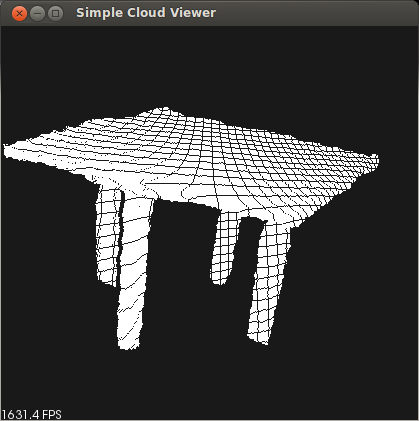
\includegraphics[width=0.30\textwidth]{figures/mesa2_1.png}
	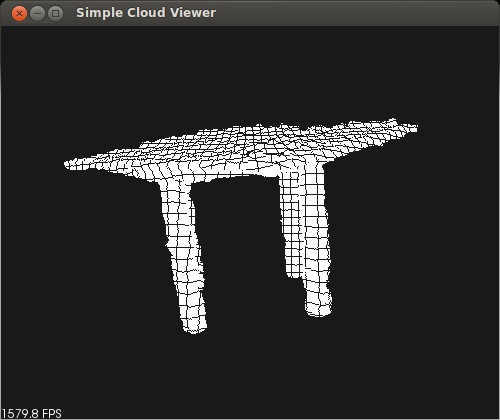
\includegraphics[width=0.30\textwidth]{figures/mesa2_2.png}
	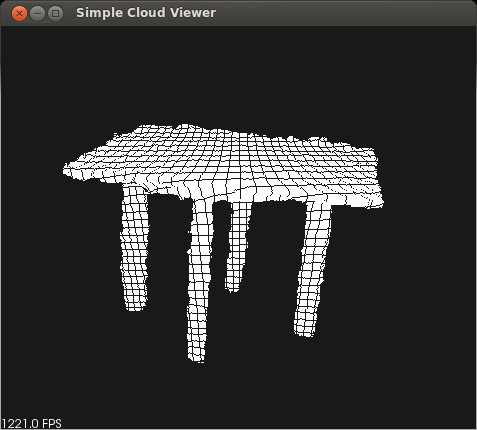
\includegraphics[width=0.30\textwidth]{figures/mesa2_3.png}
	\captionof{figure}{Clusters representativos da mesa 2.}
	\label{fig:mesa2_ensaios}
\end{center}
\end{figure}


\begin{table}[htb]
\begin{center}
\begin{tabular} { c c c c c | c }
	Modelo do dicionário & \(C_1\) & \(C_2\) & \(C_n\) & \(C_h\) & \(C\) \\
	\hline
	\multicolumn{6}{ c }{Primeiro Ensaio}\\
	\hline
	Mesa 1 &	 0.423086 &	0.664045 & 1.000000 & 0.375991 & 0.584580 \\
	Mesa 2 &	 0.596547 &	0.811000 & 1.000000 & 0.365248 & 0.661461 \\
	Mesa 3 &	 0.596547 &	0.811000 & 1.000000 & 0.433345 & 0.681890 \\
	Mesa 4 &	 0.701727 &	0.792667 & 0.666667 & 0.284082 & 0.592156 \\
	Mesa 5 &	 0.935636 &	0.792667 & -2.000000 & 0.319592 & 0.127953 \\
	\hline
	\multicolumn{6}{ c }{Segundo Ensaio}\\
	\hline
	Mesa 1 &	 0.490549 &	0.612359 & 0.750000 & 0.440277 & 0.557810 \\
	Mesa 2 &	 0.656589 &	0.765000 & 0.750000 & 0.427698 & 0.633707 \\
	Mesa 3 &	 0.656589 &	0.765000 & 0.750000 & 0.507438 & 0.657629 \\
	Mesa 4 &	 0.671706 &	0.823333 & 1.000000 & 0.332654 & 0.673556 \\
	Mesa 5 &	 0.895608 &	0.823333 & -1.000000 & 0.374236 & 0.342006 \\
	\hline
	\multicolumn{6}{ c }{Terceiro Ensaio}\\
	\hline
	Mesa 1 &	 0.610414 &	0.776405 & 1.000000 & 0.288464 & 0.633244 \\
	Mesa 2 &	 0.763269 &	0.911000 & 1.000000 & 0.280222 & 0.702634 \\
	Mesa 3 &	 0.763269 &	0.911000 & 1.000000 & 0.332467 & 0.718307 \\
	Mesa 4 &	 0.618366 &	0.726000 & 0.666667 & 0.217950 & 0.534810 \\
	Mesa 5 &	 0.824488 &	0.726000 & -2.000000 & 0.245194 & 0.061180 \\
	\hline
\end{tabular}
	\caption{Resultados da análise da Mesa 3}
	\label{res:mesa3}
\end{center}
\end{table}

O resultado desta análise \ref{res:mesa3} é também bastante satisfatório pois permite a identificação correta da mesa em análise na maioria dos casos: mesa 3.



\begin{figure}[htb]
\begin{center}
	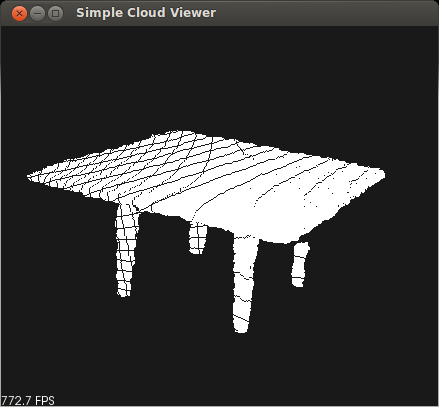
\includegraphics[width=0.30\textwidth]{figures/mesa3_1.png}
	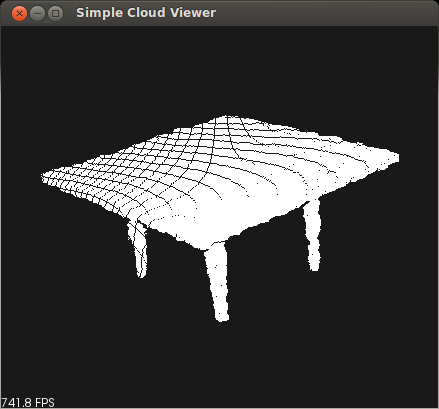
\includegraphics[width=0.30\textwidth]{figures/mesa3_2.png}
	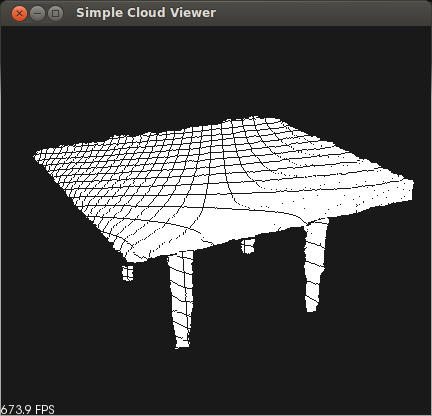
\includegraphics[width=0.30\textwidth]{figures/mesa3_3.png}
	\captionof{figure}{Clusters representativos da mesa 3.}
	\label{fig:mesa3_ensaios}
\end{center}
\end{figure}



Os resultados são satisfatórios, pois pelos dados extraídos pode-se concluir que com uma técnica de identificação bastante simples, apesar de extensível, é possível reconhecer com sucesso uma mesa, cuja morfologia tenha sido previamente guardada.
Um dos grandes defeitos é o tempo que o pré-processamento demora, que a ser melhorado permitiria o rápido reconhecimento das mesas criando uma vantagem significativa no reconhecimento de objetos complexos.


\subsection{Tempos de Processamento}

Os tempos de processamento são de extrema importância pois avaliam a adequação da solução ao âmbito da robótica autónoma, pois este requer baixos tempos de execução para fazer rapidamente a identificação de objetos.

\begin{table}[htb]
\begin{center}
\begin{tabular} { l | c c }
	\multicolumn{3}{ c }{ Tempos de processamento}\\
	Ensaio & Pré processamento (s) & Identificação (s)\\
	\hline
	1 & 11.840000 & 0.41 \\
	2 &  8.530000 & 0.40 \\
	3 & 18.770000 & 0.46 \\
	\hline
\end{tabular}
	\caption{Tempos de processamento da análise da Mesa 1}
	\label{res:mesa1_tempo}
\end{center}
\end{table}

Como se vê na tabela~\ref{res:mesa1_tempo} a maior parte do tempo de execução é passado no pré processamento, sendo a comparação com os modelos do dicionário feita de uma forma praticamente instantânea.

\begin{table}[htb]
\begin{center}
\begin{tabular} { l | c c }
	\multicolumn{3}{ c }{ Tempos de processamento}\\
	Ensaio & Pré processamento (s) & Identificação (s)\\
	\hline
	1 & 39.330000 & 1.02 \\
	2 & 13.460000 & 0.83 \\
	3 & 24.620000 & 0.74 \\
	\hline
\end{tabular}
	\caption{Tempos de processamento da análise da Mesa 2}
	\label{res:mesa2_tempo}
\end{center}
\end{table}

Verifica-se a tendência do pré-processamento ser bastante custoso, oscilando aqui entre aproximadamente 40 segundos e 13 segundos, enquanto que a identificação demora sempre aproximadamente 1 segundo.

\begin{table}[htb]
\begin{center}
\begin{tabular} { l | c c }
	\multicolumn{3}{ c }{ Tempos de processamento}\\
	Ensaio & Pré processamento (s) & Identificação (s)\\
	\hline
	1 & 35.510000 & 0.24 \\
	2 & 39.630000 & 0.24 \\
	3 & 62.590000 & 0.36 \\
	\hline
\end{tabular}
	\caption{Tempos de processamento da análise da Mesa 3}
	\label{res:mesa3_tempo}
\end{center}
\end{table}

Nos tempos de processamento para uma imagem RGBD com a Mesa 3 confirma-se que o tempo de pré processamento é bastante significativo, e apesar de absolutamente necessário acaba por atrasar o mais importante da questão que é a identificação do objeto.



%\section{Resumo}
